\subsection{Tworzenie Postaci}
Po zaprojektowaniu postaci dołączyliśmy je do naszego folderu z projektem. Żeby nasza postać pojawiła się na mapie, musimy ją przeciągnąć na wcześniej utworzoną scenę. Tak oto otrzymaliśmy nieruchomy model naszego maga. Aby upewnić się, że jest on poprawnie ulokowany, możemy sprawdzić zakładkę Hierarchy, gdzie znajdziemy listę wszystkich dostępnych obiektów na mapie. 

W naszym wypadku nie możemy jednak umieścić postaci od razu w rozgrywce, gdyż nie będzie mogła ona być poprawnie sterowana przez danego gracza. Żeby system Multiplayer działał sprawnie, musimy stworzyć tak zwanego „Prefaba”, czyli obiekt w grze, który ma pewne właściwości, może zostać wielokrotnie użyty, lub pojawić się np. w momencie zalogowania gracza do gry. W tym celu musimy przeciągnąć nasz obiekt, który ma zamienić się w typ Prefab z listy Hierarchy, do naszego folderu (W tym przypadku jest to folder Assets). Teraz w celu ulokowania naszych magów na mapie, wystarczy przeciągnąć obiekt z rozszerzeniem .prefab na naszą scenę. Przy umieszczaniu takich samych obiektów Unity automatycznie będzie dodawało do naszej nazwy numer obiektu np. Wizard (1). 
\begin{figure}[H]
	\center
	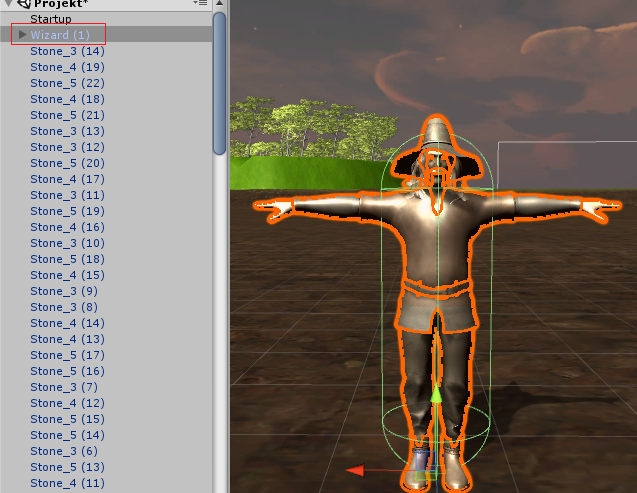
\includegraphics[width=\textwidth]{prefab.png}
	\caption{Ręczne rozwiązywanie konfliktów w projekcie gry}
\end{figure}
Jest to również bardzo dobre rozwiązanie, gdy w projekcie musimy użyć wielu takich samych obiektów. W naszej grze wykorzystaliśmy to między innymi podczas tworzenia przeciwników dla naszych graczy. Dzięki temu tworząc jeden model wroga, mogliśmy go użyć w wielu miejscach, bez konieczności tworzenia od nowa tego samego szkieletu postaci.
\begin{figure}[H]
	\center
	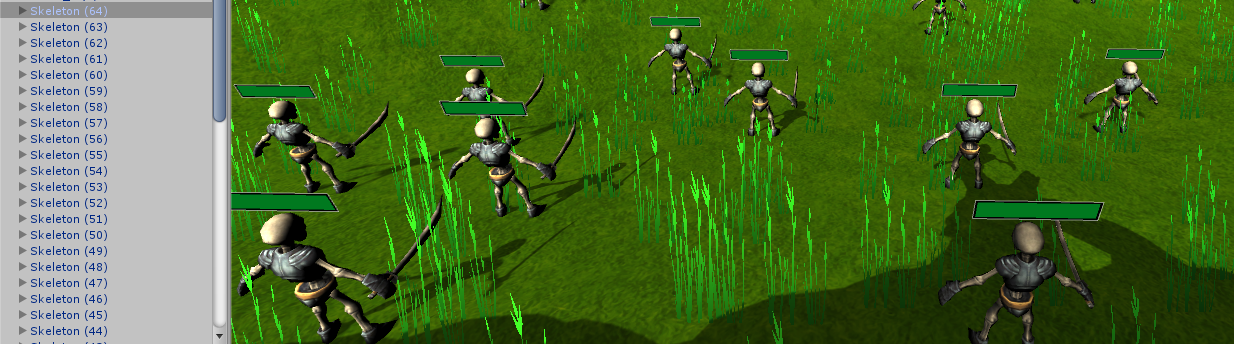
\includegraphics[width=\textwidth]{prefab2.png}
	\caption{Armia szkieletów utworzona przy pomocy jednego Prefaba}
\end{figure}

Każdy obiekt poza nazwą posiada również swój Tag, możemy dzięki temu definiować np. grupę wrogów, przedmiotów o specjalnych właściwościach lub graczy. Na przykładzie naszej gry sprawdziło się to przy wykonywaniu misji. Szkielety w mieście posiadają specjalny Tag, który wyróżnia je od pozostałych. Jeśli zostaną one pokonane, dopiero wtedy kobieta w mieście przekaże nam kolejne informacje.
\begin{figure}[H]
	\center
	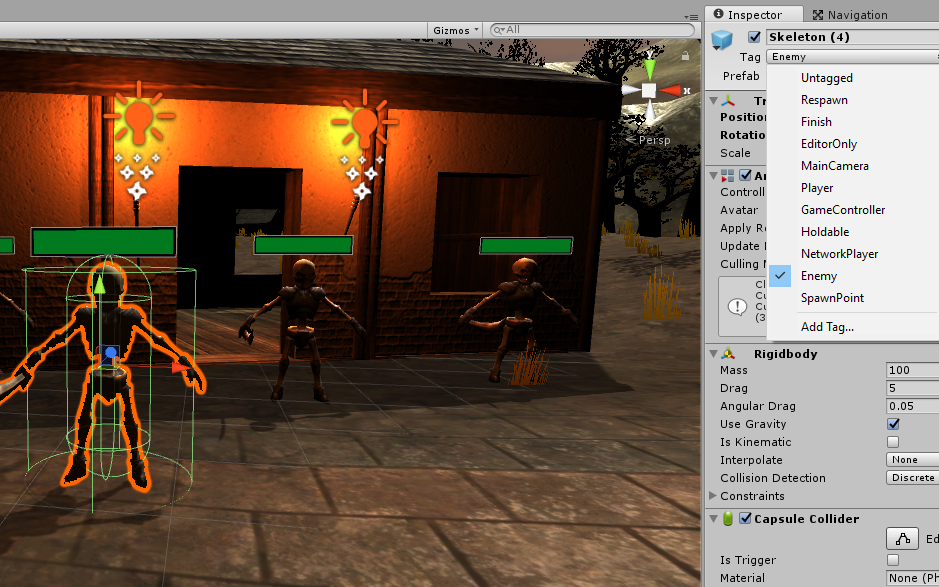
\includegraphics[width=\textwidth]{Tag.png}
	\caption{Tagi zdefiniowane w naszym projekcie, które możemy przyporządkować do danego obiektu}
\end{figure}


Bardzo istotne w obiekcie są komponenty. To one odpowiadają za to jak zachowuje się dany obiekt. Wszystkie skrypty odpowiadające za poruszanie się, grawitację oraz inne czynności ulokowane są na obiekcie pod postacią komponentów.

\begin{figure}[H]
	\center
	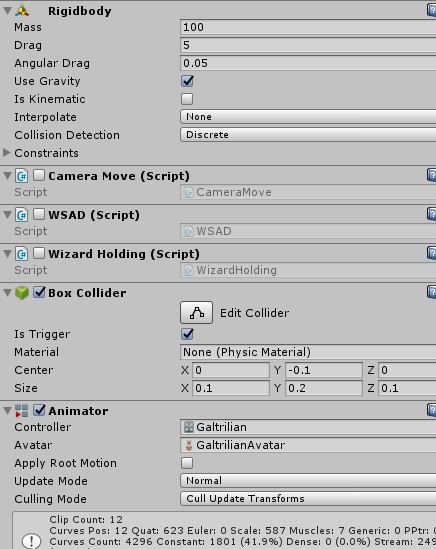
\includegraphics[width=9cm]{component.png}
	\caption{Przykładowe komponenty postaci maga odpowiadające min. za poruszanie się, kolizje z otoczeniem oraz animacje}
\end{figure}



Niektóre obiekty mogą składać się z kilku innych obiektów. Dobrym przykładem jest rycerz, który poza modelem postaci, posiada również obiekt tarczy, hełmu oraz miecza. Każdy z tych obiektów posiada również swoje własne komponenty. W przypadku miecza może być to komponent odpowiadający za wykrywanie kolizji z przeciwnikiem i tym samym odbieraniem mu odpowiedniej ilości zdrowia, gdy zostanie trafiony.
